\documentclass[12pt]{article}
\usepackage{times} 			% use Times New Roman font

\usepackage[margin=1in]{geometry}   % sets 1 inch margins on all sides
\usepackage{hyperref}               % for URL formatting
\usepackage[pdftex]{graphicx}       % So includegraphics will work
\setlength{\parskip}{1em}           % skip 1em between paragraphs
\usepackage{indentfirst}            % indent the first line of each paragraph
\usepackage{datetime}
\usepackage[small, bf]{caption}
\usepackage{listings}               % for code listings
\usepackage{xcolor}                 % for styling code
\usepackage{multirow}
\usepackage{xurl} 
\usepackage{enumitem}
\usepackage[section]{placeins}
\usepackage{float}
\usepackage{hyperref}

%New colors defined below
\definecolor{backcolour}{RGB}{246, 246, 246}   % 0xF6, 0xF6, 0xF6
\definecolor{codegreen}{RGB}{16, 124, 2}       % 0x10, 0x7C, 0x02
\definecolor{codepurple}{RGB}{170, 0, 217}     % 0xAA, 0x00, 0xD9
\definecolor{codered}{RGB}{154, 0, 18}         % 0x9A, 0x00, 0x12

%Code listing style named "gcolabstyle" - matches Google Colab
\lstdefinestyle{gcolabstyle}{
  basicstyle=\ttfamily\small,
  backgroundcolor=\color{backcolour},   
  commentstyle=\itshape\color{codegreen},
  keywordstyle=\color{codepurple},
  stringstyle=\color{codered},
  numberstyle=\ttfamily\footnotesize\color{darkgray}, 
  breakatwhitespace=false,         
  breaklines=true,                 
  captionpos=b,                    
  keepspaces=true,                 
  numbers=left,                    
  numbersep=5pt,                  
  showspaces=false,                
  showstringspaces=false,
  showtabs=false,                  
  tabsize=2
}

\lstset{style=gcolabstyle}      %set gcolabstyle code listing

\makeatletter
\g@addto@macro{\UrlBreaks}{\UrlOrds}
\makeatother

% for fancy page headings
\usepackage{fancyhdr}
\setlength{\headheight}{13.6pt} % to remove fancyhdr warning
\pagestyle{fancy}
\fancyhf{}
\rhead{\small \thepage}
\lhead{\small HW4, Lewis}  
\chead{\small CS 432, Fall 2020} 

%-------------------------------------------------------------------------
\begin{document}

\begin{centering}
{\large\textbf{HW4 - Exploring Social Networks}}

Brenden Lewis\\                     
Due: 10/25/2020 11:59PM\\                      
\end{centering}

%-------------------------------------------------------------------------
\section*{Q1}

The code for Because I find it easier to work with dictionaries in regards to storing data for individuals, I read in each 'friend' entry from \emph{HW4-friend-count.csv} as a dictionary containing their name and number of friends, and stored them in an list which was then sorted before any calculations were made. I utilized the \emph{statistics} package to calculate the mean, median, and standard deviation of the friend counts (\emph{statistics} is used for the same calculations for the other questions).

\lstinputlisting[language=Python, caption=Python code Q1, label=lst:import]{q1.py}

\par Listing 2 shows the output of the calculations for Q1. I'm a little skeptical of the result for standard deviation as it seems a bit too high; this could be due to outliers in the data, or an error in calculating the standard deviation (either wrong methods or some other factor I'm missing).

\begin{lstlisting}[language=Python, caption={Calculated mean, median, and standard deviation for Q1}, label=lst:copy]
Statistics for 'Friend' counts of U and their friends
Mean: 538
Median: 395
Standard Deviation: 535.81
\end{lstlisting}

\par Figure 1 shows a scatter plot of the User's (U) friend counts compared to their friends' friend counts. The results of graph seem to show that the Friendship Paradox holds for this particular user. The User had about 98 friends in their list. Compared to the majority of their friends, the User has a lot less friends, with some friends having thousands more friends to their account.

\begin{figure}
    \centering
    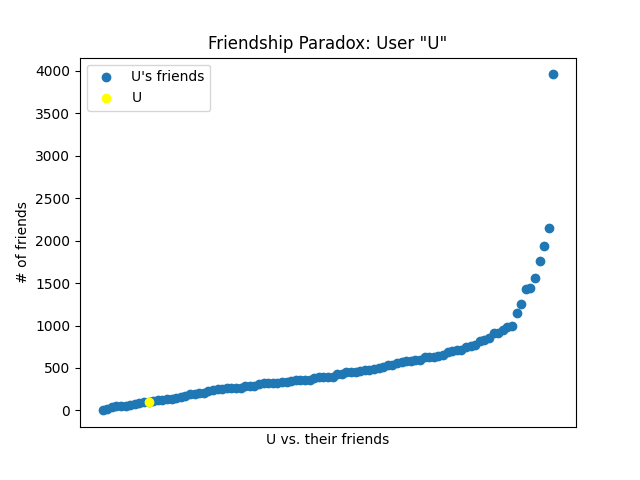
\includegraphics{Q1_Graph.png}
    \caption{Graph showing the friend count of the user, and the friend counts of their friends}
    \label{fig:my_label}
\end{figure}

\section*{Q2}

I opted to split this section into two programs: one to collect all the follower counts from Twitter (Listing 3), and one to handle data calculations and graphing (Listing 5). I don't have an active Twitter account, so I used our instructor's Twitter handle \emph{'weiglemc'} as the user ID to collect data. The biggest challenge here was handling a RateLimitError that occured when the rate limit was exceeded pulling from Twitter. I got around this by adding the parameter \emph{wait\textunderscore rate\textunderscore limit=True} to the \emph{api} initialization. This caused the stream to halt when the rate limit was reached to give it time to refresh and prevent errors from attempting to exceed it. 

\par A Cursor was used to move through the list of \emph{weiglemc}'s followers. For each follower, a dictionary was created with their Twitter handle (ID) and their follower counts and stored in list which would then be sorted by follower counts after everyone was processed; follower counts was found using \emph{'.followers\textunderscore count'} for each user.

\emph{Of note: I ended up not using the getFollowerCount() method and forgot to remove it.}

\lstinputlisting[language=Python, caption=Python code Q2, label=lst:import]{q2.py}

Listing 4 below shows how the information for each user was stored in the output file:

\begin{lstlisting}[language=Python, caption={Examples of stored dictionaries for followers}, label=lst:copy]
{'USER': 'rachelheldevans', 'FOLLOWERCOUNT': 163355}
{'USER': 'KHayhoe', 'FOLLOWERCOUNT': 169495}
{'USER': 'mattcutts', 'FOLLOWERCOUNT': 529815}
\end{lstlisting}

Listing 5 below is a slightly modified version of the code from Listing 1 to accomodate the data collected for Q2. The only major difference aside from file and graph nomenclature is how the information from the new file is read in. Listing 1 uses a method \emph{csv.DictReader()} from the \emph{csv} library to read in lines from csv files as dictionaries. Listing 5 (and also Listing 10 for Q3) uses \emph{ast.literal\textunderscore eval(line)} to convert each line from the file, as is, into a dictionary to be stored. The users were already sorted previously, so there was no need to sort again.

\lstinputlisting[language=Python, caption=Python code for graphing follower counts, label=lst:import]{graphFollowers.py}

\par Listing 6 shows the output for calculations using data from follower counts. Listing 7 shows the output from the same data minus three outliers heavily skewing the data to the right. The errors related to standard deviation seem much more apparent in these listings compared to that in Q1, or once again the deviation is being affected by the larger follower counts skewing the data. It remains unclear.

\begin{lstlisting}[language=Python, caption={Calculated mean, median, and standard deviation for Q2}, label=lst:copy]
Statistics for 'Follower' counts of weiglemc and their followers
Mean: 2915
Median: 195
Standard Deviation: 27839.99
\end{lstlisting}

\begin{lstlisting}[language=Python, caption={Calculated mean, median, and standard deviation for Q2, excluding a few outliers}, label=lst:copy]
Statistics for 'Follower' counts of weiglemc and their followers
Mean: 945
Median: 393
Standard Deviation: 2244.33
\end{lstlisting}

Figure 2 shows the original data of the user \emph{weiglemc}'s followers, and their followers' followers. To help provide a better visual curve, the three outliers were removed and the data was graphed again in Figure 3. It is difficult to tell based on both graphs if the Friendship Paradox holds as \emph{weiglemc} is just a little right of the middle of both curves; this would indicate that \emph{weiglemc} has more followers than more than half of the users they follow.

\begin{figure}
    \centering
    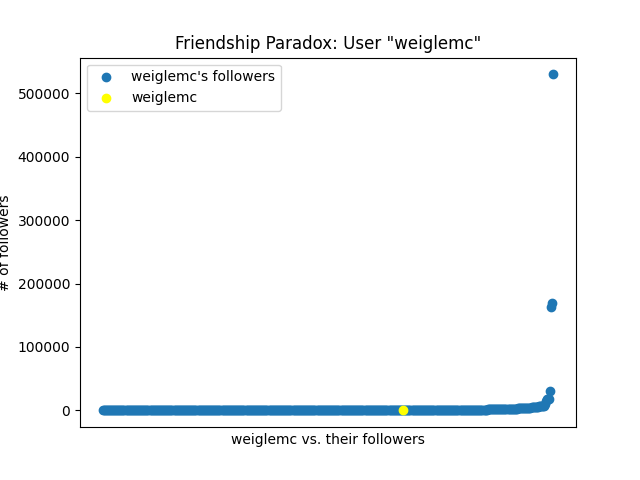
\includegraphics{FollowerCounts.png}
    \caption{Graph showing the follower count of the user, and the follower counts of their followers}
    \label{fig:my_label}
\end{figure}


\begin{figure}
    \centering
    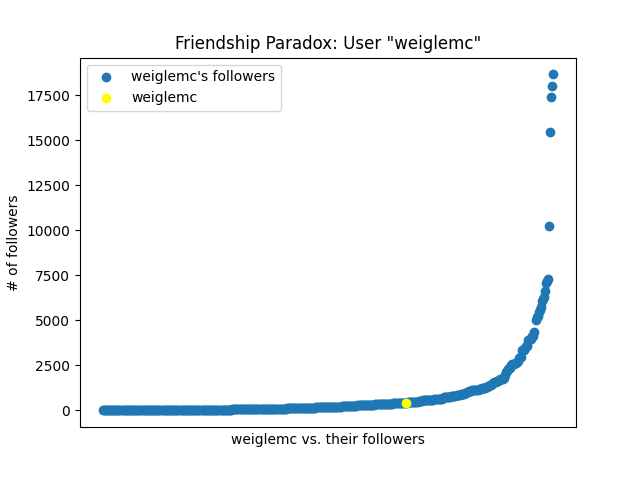
\includegraphics{FollowerCountsTrimmed.png}
    \caption{Graph showing the follower count of the user, and the follower counts of their followers, excluding outliers}
    \label{fig:my_label}
\end{figure}

\section*{Q3 (Extra)}

The code used for Q3 (Listing 8 and 10) is very much the same to that used in Q2 with a few minor changes. In order to get \emph{following} counts from a user instead of \emph{followers}, I had to alter the Cursor to use \emph{api.friends} and call \emph{.friends\textunderscore count} for each user to get the number of users they each follow. For some reason, the Twitter API uses Friend interchangeably with Follower when doing anything related to who a user follows. When collecting data, I had to double check a few Twitter accounts to ensure it was actually capturing the number of users they follow.  

\lstinputlisting[language=Python, caption=Python code Q3, label=lst:import]{q3.py}

Listing 9 shows how the data gathered was stored in the output file before any calculations or graphing is done.

\begin{lstlisting}[language=Python, caption={Examples of stored dictionaries for accounts followed}, label=lst:copy]
{'USER': 'nakedpastor', 'FRIENDCOUNT': 17790}
{'USER': 'MarkWarner', 'FRIENDCOUNT': 25114}
{'USER': 'BarackObama', 'FRIENDCOUNT': 599538}
\end{lstlisting}


\lstinputlisting[language=Python, caption=Python code for graphing following counts, label=lst:import]{graphFriends.py}

Listing 11 shows the results of calculations of data collected for Q3. Listing 12 shows the same data exluding a single outlier that was \emph{very} heavily skewing the data, the account of late President Barack Obama with nearly six-hundred thousand accounts followed.

\begin{lstlisting}[language=Python, caption={Calculated mean, median, and standard deviation for Q3}, label=lst:copy]
Statistics for 'Following' counts of weiglemc and who they follow
Mean: 3238
Median: 394
Standard Deviation: 37048.7
\end{lstlisting}

\begin{lstlisting}[language=Python, caption={Calculated mean, median, and standard deviation for Q3, excluding an outlier}, label=lst:copy]
Statistics for 'Following' counts of weiglemc and who they follow
Mean: 859
Median: 192
Standard Deviation: 2094.13
\end{lstlisting}

Figures 4 and 5 show scatter plots of the data for Q3, with Figure 5 excluding Obama's account to get a more accurate visual. In the case of \emph{weiglemc}, just like in Q2, it is difficult to tell if the Friendship Paradox holds for counts of users followed as they are placed very near the center of the curves. User \emph{weiglemc} veers slightly to the left of the median, meaning they are following less users than more than 50\% of the users they follow.

\begin{figure}
    \centering
    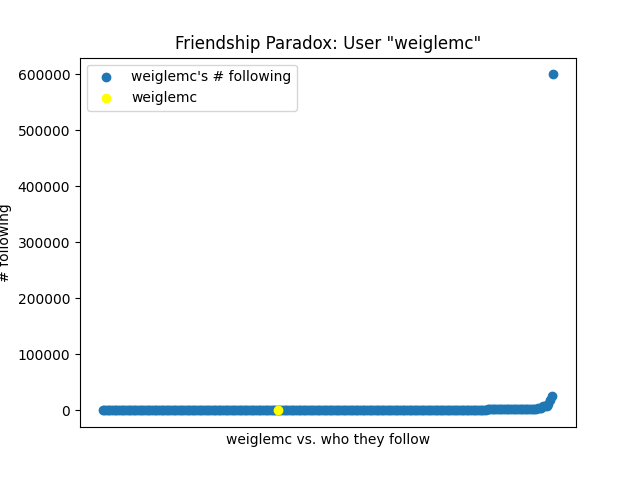
\includegraphics{FollowingCounts.png}
    \caption{Graph showing the number of accounts the user follows, and the following counts of those they follow}
    \label{fig:my_label}
\end{figure}

\begin{figure}
    \centering
    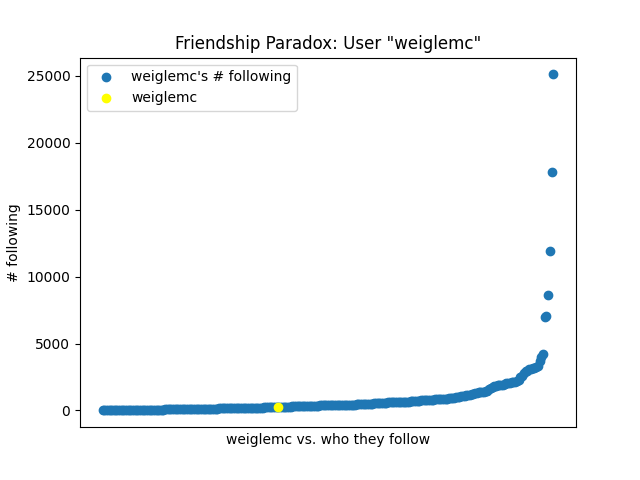
\includegraphics{FollowingCountsTrimmed.png}
    \caption{Graph showing the number of accounts the user follows, and the following counts of those they follow, excluding outliers}
    \label{fig:my_label}
\end{figure}

\end{document}
